\section{Progettazione di Dettaglio e Codifica}
\textit{Dal 2021-03-08 al 2021-04-09}

\begin{figure}[H]
	\centering
	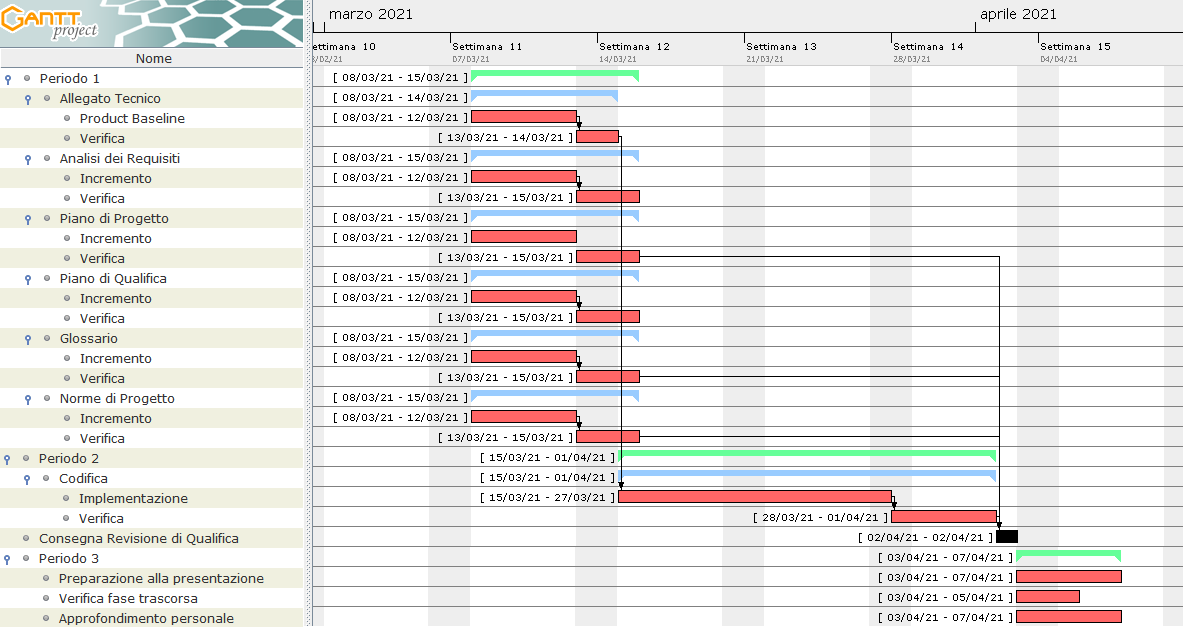
\includegraphics[scale=0.48]{res/images/gantt_fase/04_gantt_codifica_obbligatori.png}
	\caption{Diagramma di Gantt\textsubscript{G} relativo alla Progettazione e Codifica}
\end{figure}


\subsection{Periodo 1}

\subsubsection{Pianificazione preventiva}

\paragraph{Attività}
\subparagraph*{}

\planningTable{
	Allegato Tecnico & Viene integrato l'\textsc{Allegato Tecnico}, che presenterà ora anche la Product Baseline, nella quale il software è scomposto e analizzato nelle sue unità. & 40 & Progettista
\tabularnewline 
Incremento Analisi dei Requisiti & L'avanzamento nello sviluppo del prodotto chiarirà alcuni aspetti che nella fase\textsubscript{G} di Analisi risultavano oscuri, e potrebbe evidenziare delle criticità non inizialmente considerate. Se necessario, viene raffinata l'\textsc{Analisi dei Requisiti}. & 6 & Analista
\tabularnewline 
Incremento Piano di Progetto & Il \textsc{Piano di Progetto} integrato con il consuntivo del periodo\textsubscript{G} trascorso & 3 & Responsabile
\tabularnewline 
Incremento Glossario & Viene integrato con nuovi termini. & 1 & Responsabile
\tabularnewline 
Incremento Piano di Qualifica & Il cruscotto\textsubscript{G} viene aggiornato con i dati rilevati sul periodo\textsubscript{G} trascorso & 8 & Verificatore
\tabularnewline 
\caption{Pianificazione preventiva - Progettazione di Dettaglio e Codifica - Periodo 1}
}

\paragraph{Preventivo}
\subparagraph*{}

\hspace{-1cm}
\begin{minipage}{.50\textwidth}
\smallPreventivoTable{
	Responsabile & 4 & 120\\ 
Verificatore & 8 & 120\\ 
Analista & 6 & 150\\ 
Amministratore & 0 & 0\\ 
Programmatore & 0 & 0\\ 
Progettista & 40 & 880\\ 
\hlinetable 
\textbf{Totale} & \textbf{58} & \textbf{1270}\\ 
\end{tabular} 
\caption{Progettazione di Dettaglio e Codifica - Periodo 1}
}
\end{minipage}
\hspace{1cm}
\begin{minipage}{.40\textwidth}
\begin{figure}[H]
	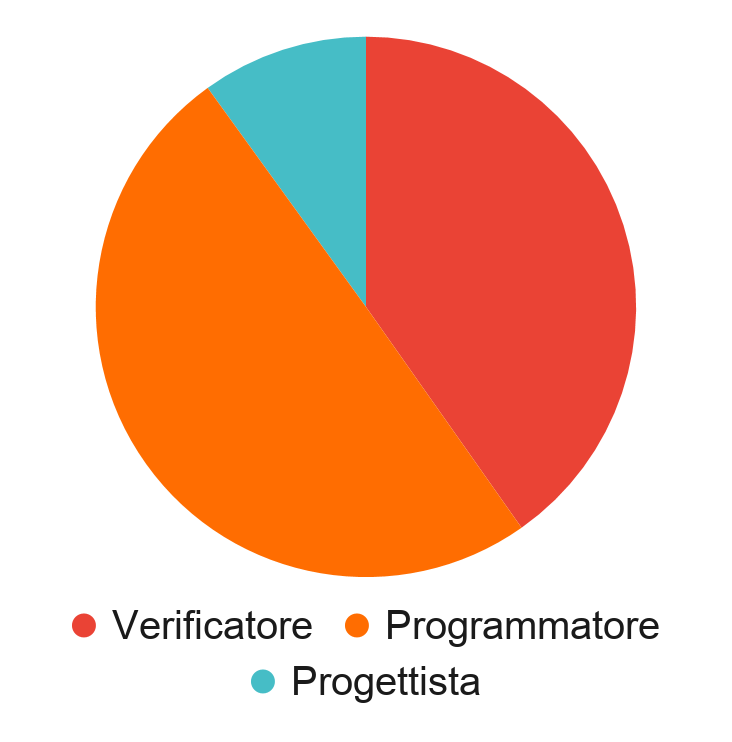
\includegraphics[scale=0.21]{res/images/charts/preventivo_priori/Grafico4-6.png}
	\caption{Distribuzione dei costi: preventivo - Progettazione di Dettaglio e Codifica - Periodo 1}
\end{figure}
\end{minipage} 



\subsubsection{Pianificazione di periodo}

%TODO: NICOLO'
%\begin{figure}[H]
%	\centering
%	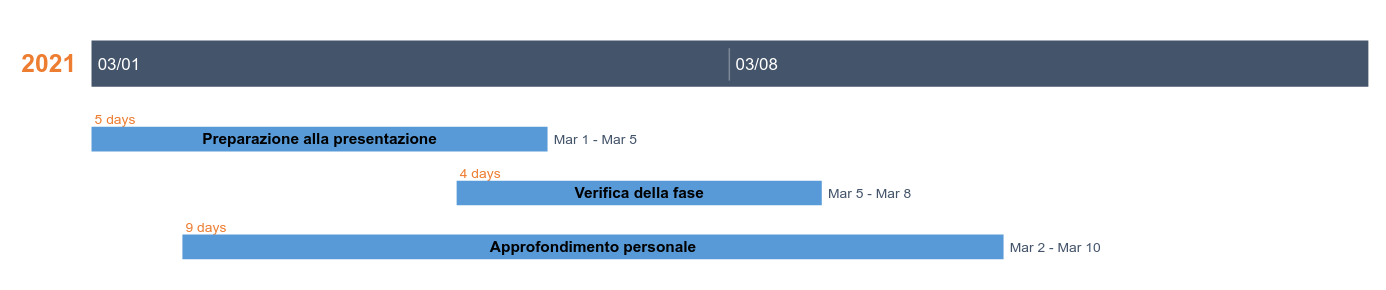
\includegraphics[scale=0.30]{res/images/gantt_periodo/progarch_3_gantt.png}
%	\caption{Gantt di periodo\textsubscript{G} - Progettazione di Dettaglio e Codifica - Periodo 1}
%\end{figure}

\paragraph{Attività}
\subparagraph*{}

\planningTable{
	Allegato Tecnico (PB) & Viene studiata e formalizzata l'architettura del software. La progettazione confluisce nella Product Baseline. & 30 & Progettista
\tabularnewline 
Incremento Analisi dei Requisiti & L'avanzamento nello sviluppo del prodotto chiarirà alcuni aspetti che nell'Analisi risultavano oscuri, e potrebbe evidenziare delle criticità non inizialmente considerate. Se necessario, viene raffinata l'\textsc{Analisi dei Requisiti}. & 2 & Analista
\tabularnewline 
Incremento Piano di Progetto & Il \textsc{Piano di Progetto} integrato con il consuntivo del periodo\textsubscript{G} trascorso. & 2 & Responsabile
\tabularnewline 
Incremento Glossario & Viene integrato con nuovi termini. & 1 & Responsabile
\tabularnewline 
Incremento Piano di Qualifica & Il cruscotto\textsubscript{G} viene aggiornato con i dati rilevati sul periodo\textsubscript{G} trascorso. & 4 & Verificatore
\tabularnewline 
Incremento Norme di Progetto & Le Norme di Progetto vengono incrementate con le norme per la codifica. & 1 & Amministratore
\tabularnewline 
\caption{Pianificazione di periodo\textsubscript{G} - Progettazione di Dettaglio e Codifica - Periodo 1}
}



\paragraph{Preventivo orario ed economico}
\subparagraph*{}

\contabilitaTable{
	Chiarello Sofia & 0 & 0 & 1 & 0 & 0 & 5 & \textbf{6}\\ 
Crivellari Alberto & 0 & 2 & 0 & 0 & 0 & 5 & \textbf{7}\\ 
De Renzis Simone & 2 & 0 & 0 & 0 & 0 & 5 & \textbf{7}\\ 
Greggio Nicolò & 1 & 0 & 0 & 1 & 0 & 5 & \textbf{7}\\ 
Tessari Andrea & 0 & 2 & 0 & 0 & 0 & 5 & \textbf{7}\\ 
Zuccolo Giada & 0 & 0 & 1 & 0 & 0 & 5 & \textbf{6}\\ 
\hlinetable 
\textbf{Totale orario} & \textbf{3} & \textbf{4} & \textbf{2} & \textbf{1} & \textbf{0} & \textbf{30} & \textbf{40}\\ 
\textbf{Totale costo} & \textbf{90} & \textbf{60} & \textbf{50} & \textbf{20} & \textbf{0} & \textbf{660} & \textbf{880}\\ 
\end{tabular} 
\caption{Preventivo di periodo - Progettazione di Dettagli e Codifica - Periodo 1}
}

\begin{figure}[H]
	\centering
	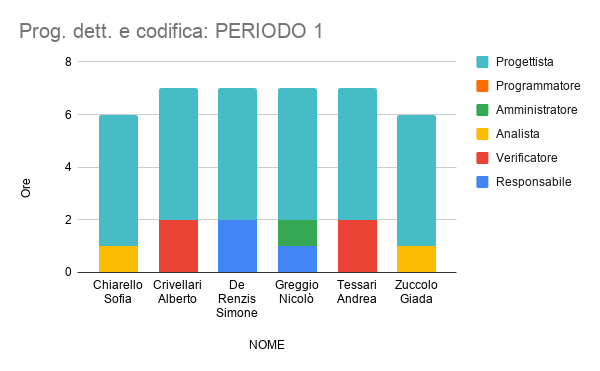
\includegraphics[scale=0.6]{res/images/charts/preventivo/prog_dett_1.png}
	\caption{Distribuzione oraria per componente: preventivo di periodo\textsubscript{G} - Progettazione di Dettaglio e Codifica - Periodo 1}
\end{figure}



\subsubsection{Riscontro di fine periodo}


\paragraph{Consuntivo orario ed economico}
\subparagraph*{}

\contabilitaTable{
	Chiarello Sofia & 0 & 0 & 1 & 0 & 0 & 5 & \textbf{6} \\ 
Crivellari Alberto & 0 & 3 & 0 & 0 & 0 & 5 & \textbf{8} \\ 
De Renzis Simone & 1 & 0 & 0 & 0 & 0 & 6 & \textbf{7} \\ 
Greggio Nicolò & 1 & 0 & 0 & 1 & 0 & 5 & \textbf{7} \\ 
Tessari Andrea & 0 & 2 & 0 & 0 & 0 & 6 & \textbf{8} \\ 
Zuccolo Giada & 0 & 0 & 1 & 0 & 0 & 5 & \textbf{6} \\ 
\hlinetable 
\textbf{Totale orario} & \textbf{2} & \textbf{5} & \textbf{2} & \textbf{1} & \textbf{0} & \textbf{32} & \textbf{42} \\ 
\textbf{Differenza orario} & \textbf{-1} & \textbf{1} & \textbf{0} & \textbf{0} & \textbf{0} & \textbf{2} & \textbf{2} \\ 
\textbf{Totale costi} & \textbf{60} & \textbf{75} & \textbf{50} & \textbf{20} & \textbf{0} & \textbf{704} & \textbf{909} \\ 
\textbf{Differenza costi} & \textbf{-30} & \textbf{15} & \textbf{0} & \textbf{0} & \textbf{0} & \textbf{44} & \textbf{29} \\ 
\end{tabular} 
\caption{Consuntivo - Progettazione di Dettaglio e Codifica - Periodo 1}
}

\begin{figure}[H]
	\centering
	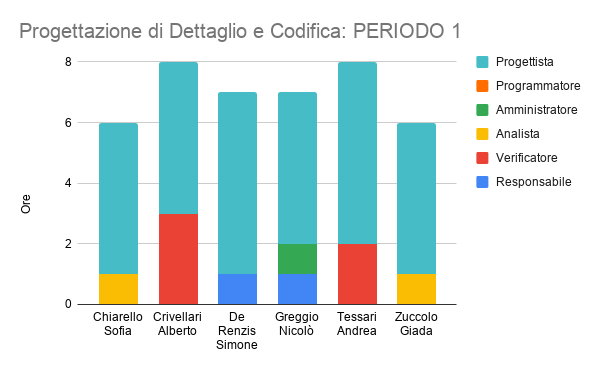
\includegraphics[scale=0.6]{res/images/charts/consuntivo/prog_dett_1.png}
	\caption{Distribuzione oraria per componente: consuntivo - Progettazione di Dettaglio e Codifica - Periodo 1}
\end{figure}


Il periodo\textsubscript{G} chiude in \textbf{negativo}, costringendo ad una spesa supplementare di \textbf{29 \euro} rispetto a quando preventivato all'inizio del periodo\textsubscript{G}. Tuttavia è apprezzabile la riduzione dei costi rispetto a quanto preventivato all'inizio del progetto per questo periodo (risparmio di \textbf{390 \euro}).


\paragraph{Preventivo a finire}
\subparagraph*{}

\pafTable{
	Avvio & 1 & Consuntivo & 1060
\tabularnewline
Analisi dei Requisiti & 1 & Consuntivo & 3380
\tabularnewline
Analisi dei Requisiti & 2 & Consuntivo & 255
\tabularnewline
Progettazione Architetturale & 1 & Consuntivo & 2220
\tabularnewline
Progettazione Architetturale & 2 & Consuntivo & 2000
\tabularnewline
Progettazione Architetturale & 3 & Consuntivo & 150
\tabularnewline
Progettazione di Dettaglio e Codifica & 1 & Consuntivo & 909
\tabularnewline
Progettazione di Dettaglio e Codifica & 2 & Preventivo di periodo & 2743
\tabularnewline
Progettazione di Dettaglio e Codifica & 3 & Preventivo & 258
\tabularnewline
Validazione e Collaudo & 1 & Preventivo & 220
\tabularnewline
Validazione e Collaudo & 2 & Preventivo & 2145
\tabularnewline
Validazione e Collaudo & 3 & Preventivo & 60
\tabularnewline
\textbf{Totale} & \textbf{} & \textbf{} & \textbf{15400}
\tabularnewline
\textbf{Totale rendicontato} & \textbf{} & \textbf{} & \textbf{10705}
\tabularnewline
\caption{Preventivo a finire - Progettazione di Dettaglio e Codifica - Periodo 1}
}

Grazie alle riduzioni di ore operate in questo periodo, è stato possibile rientrare nella pianificazione iniziale.


\pagebreak
\subsection{Periodo 2}

\subsubsection{Pianificazione preventiva}

\paragraph{Attività}
\subparagraph*{}

\planningTable{
	Incremento 1 & Implementazione sistema di autenticazione per i gestori del magazzino. & 20 & Progettista, Programmatore, Verificatore
\tabularnewline 
Incremento 2.A & Aggiunta possibilità di guida manuale dei muletti. & 10 & Progettista, Programmatore, Verificatore
\tabularnewline 
Incremento 2.B & Implementazione di un algoritmo efficiente per la ricerca del miglior percorso per raggiungere la destinazione. & 15 & Progettista, Programmatore, Verificatore
\tabularnewline 
Incremento 2.C & Realizzazione di un algoritmo per la rilevazione e gestione delle collisioni tra le unità. & 20 & Progettista, Programmatore, Verificatore
\tabularnewline 
Incremento 3 & Implentazione dei sensi di percorrenza nella mappa. & 10 & Progettista, Programmatore, Verificatore
\tabularnewline 
Incremento 4.A & Presentazione della mappa del magazzino tramite interfaccia realizzata in Angular.js. & 30 & Progettista, Programmatore, Verificatore
\tabularnewline 
Incremento 4.B & Ideazione e implementazione tool di creazione e modifica della mappa. & 35 & Progettista, Programmatore, Verificatore
\tabularnewline 
Incremento 4.C & Realizzazione pannello di guida dell'unità nell'interfaccia grafica, e finestra di visualizzazione delle task delle unità. & 20 & Progettista, Programmatore, Verificatore
\tabularnewline 
Incremento 4.D & Realizzazione pannello di visualizzazione delle task da svolgere e completate. & 10 & Progettista, Programmatore, Verificatore
\tabularnewline 
Incremento 5.A & Collegamento tra server, frontend e unità. & 20 & Progettista, Programmatore, Verificatore
\tabularnewline 
Incremento 5.B & Studio e applicazione di Containter Docker alle componenti del sistema. & 20 & Progettista, Programmatore, Verificatore
\tabularnewline 
Incremento 6 (opzionale) & Implementazione della velocità modulabile delle unità. & 15 & Progettista, Programmatore, Verificatore
\tabularnewline 
Incremento 7 (opzionale) & Aggiunta e implementazione di attore "pedone". & 30 & Progettista, Programmatore, Verificatore
\tabularnewline 
\caption{Pianificazione preventiva - Progettazione di Dettaglio e Codifica - Periodo 2}
}

\paragraph{Preventivo}
\subparagraph*{}

\hspace{-1cm}
\begin{minipage}{.50\textwidth}
\smallPreventivoTable{
	Responsabile & 0 & 0\\ 
Verificatore & 105 & 1575\\ 
Analista & 0 & 0\\ 
Amministratore & 0 & 0\\ 
Programmatore & 130 & 1950\\ 
Progettista & 26 & 572\\ 
\hlinetable 
\textbf{Totale} & \textbf{261} & \textbf{4097}\\ 
\end{tabular} 
\caption{Progettazione di Dettaglio e Codifica - Periodo 2}
}
\end{minipage}
\hspace{1cm}
\begin{minipage}{.40\textwidth}
\begin{figure}[H]
	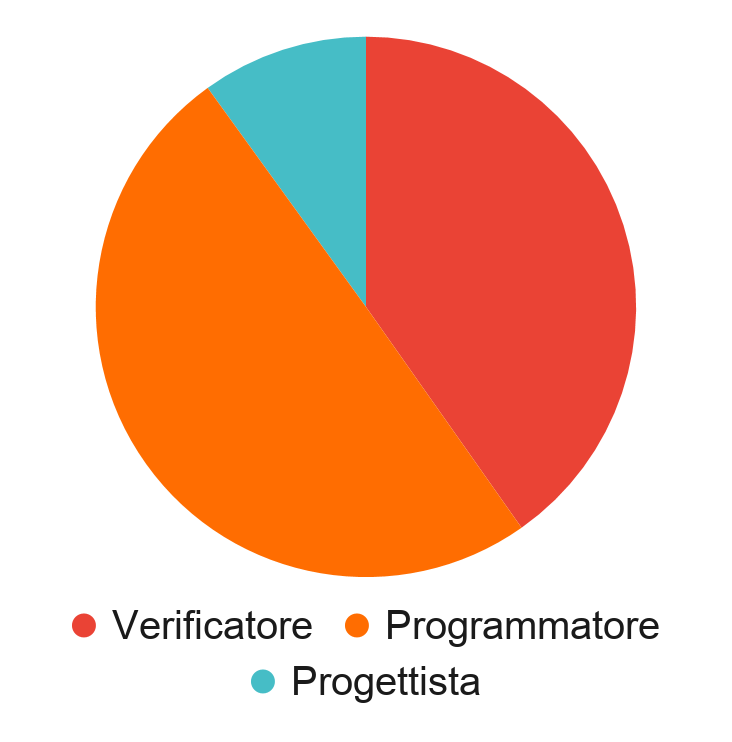
\includegraphics[scale=0.21]{res/images/charts/preventivo_priori/Grafico4-7.png}
	\caption{Distribuzione dei costi: preventivo - Progettazione di Dettaglio e Codifica - Periodo 2}
\end{figure}
\end{minipage} 




\subsubsection{Pianificazione di periodo}

%TODO: NICOLO'
%\begin{figure}[H]
%	\centering
%	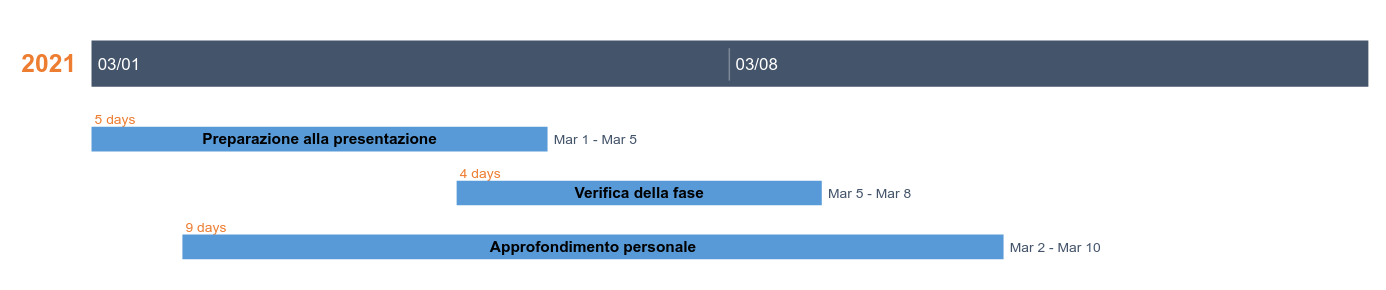
\includegraphics[scale=0.30]{res/images/gantt_periodo/progarch_3_gantt.png}
%	\caption{Gantt di periodo\textsubscript{G} - Progettazione di Dettaglio e Codifica - Periodo 2}
%\end{figure}

\paragraph{Attività}
\subparagraph*{}

\planningTable{
	Manuale Manutentore & L'architettura elaborata con la Product Baseline confluisce nel Manuale del Manutentore, che contiene anche le informazioni necessarie all'estensione del software. & 3 & Progettista
\tabularnewline 
Incremento 1 & Implementazione sistema di autenticazione per i gestori del magazzino. & 15 & Progettista, Programmatore, Verificatore
\tabularnewline 
Incremento 2.A & Aggiunta possibilità di guida manuale dei muletti. & 5 & Progettista, Programmatore, Verificatore
\tabularnewline 
Incremento 2.B & Implementazione di un algoritmo efficiente\textsubscript{G} per la ricerca del miglior percorso per raggiungere la destinazione. & 10 & Progettista, Programmatore, Verificatore
\tabularnewline 
Incremento 2.C & Realizzazione di un algoritmo per la rilevazione e gestione delle collisioni tra le unità. & 15 & Progettista, Programmatore, Verificatore
\tabularnewline 
Incremento 3 & Implentazione dei sensi di percorrenza\textsubscript{G} nella mappa. & 5 & Progettista, Programmatore, Verificatore
\tabularnewline 
Incremento 4.A & Presentazione della mappa del magazzino tramite interfaccia realizzata in Angular.js. & 25 & Progettista, Programmatore, Verificatore
\tabularnewline 
Incremento 4.B & Ideazione e implementazione tool di creazione e modifica della mappa. & 30 & Progettista, Programmatore, Verificatore
\tabularnewline 
Incremento 4.C & Realizzazione pannello di guida dell'unità nell'interfaccia grafica, e finestra di visualizzazione delle task\textsubscript{G} delle unità. & 15 & Progettista, Programmatore, Verificatore
\tabularnewline 
Incremento 4.D & Realizzazione pannello di visualizzazione delle task\textsubscript{G} da svolgere e completate. & 5 & Progettista, Programmatore, Verificatore
\tabularnewline 
Incremento 5.A & Collegamento tra server, frontend e unità. & 15 & Progettista, Programmatore, Verificatore
\tabularnewline 
Incremento 5.B & Studio e applicazione di Containter Docker alle componenti del sistema. & 15 & Progettista, Programmatore, Verificatore
\tabularnewline 
Manuale Utente & Viene redatto il \textsc{Manuale Utente}, che prevede le informazioni per installare e usufruire al meglio del software. & 10 & Progettista
\tabularnewline 
\caption{Pianificazione di periodo\textsubscript{G} - Progettazione di Dettaglio e Codifica - Periodo 2}
}



\paragraph{Preventivo orario ed economico}
\subparagraph*{}

\contabilitaTable{
	Chiarello Sofia & 0 & 4 & 0 & 0 & 18 & 6 & \textbf{28}\\ 
Crivellari Alberto & 0 & 4 & 0 & 0 & 17 & 6 & \textbf{27}\\ 
De Renzis Simone & 0 & 4 & 0 & 0 & 18 & 6 & \textbf{28}\\ 
Greggio Nicolò & 0 & 4 & 0 & 0 & 18 & 6 & \textbf{28}\\ 
Tessari Andrea & 0 & 2 & 0 & 0 & 20 & 6 & \textbf{28}\\ 
Zuccolo Giada & 0 & 4 & 0 & 0 & 20 & 4 & \textbf{28}\\ 
\hlinetable 
\textbf{Totale orario} & \textbf{0} & \textbf{22} & \textbf{0} & \textbf{0} & \textbf{111} & \textbf{34} & \textbf{167}\\ 
\textbf{Totale costo} & \textbf{0} & \textbf{330} & \textbf{0} & \textbf{0} & \textbf{1665} & \textbf{748} & \textbf{2743}\\ 
\end{tabular} 
\caption{Preventivo di periodo - Progettazione di Dettagli e Codifica - Periodo 2}
}

\begin{figure}[H]
	\centering
	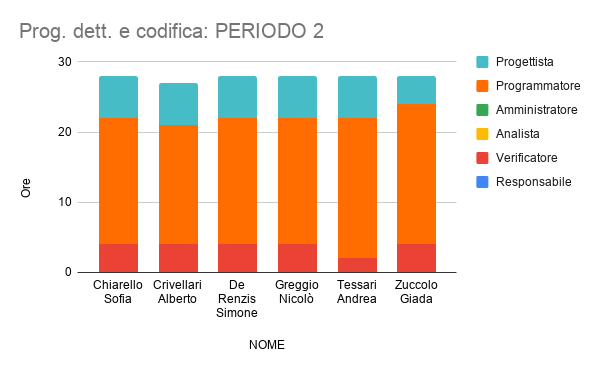
\includegraphics[scale=0.6]{res/images/charts/preventivo/prog_dett_2.png}
	\caption{Distribuzione oraria per componente: preventivo di periodo\textsubscript{G} - Progettazione di Dettaglio e Codifica - Periodo 2}
\end{figure}



\subsubsection{Riscontro di fine periodo}


\paragraph{Consuntivo orario ed economico}
\subparagraph*{}

\contabilitaTable{
	Chiarello Sofia & 0 & 4 & 0 & 0 & 18 & 5 & \textbf{27} \\ 
Crivellari Alberto & 0 & 7 & 0 & 0 & 16 & 5 & \textbf{28} \\ 
De Renzis Simone & 0 & 3 & 0 & 0 & 20 & 5 & \textbf{28} \\ 
Greggio Nicolò & 0 & 4 & 0 & 0 & 18 & 6 & \textbf{28} \\ 
Tessari Andrea & 0 & 2 & 0 & 0 & 20 & 5 & \textbf{27} \\ 
Zuccolo Giada & 0 & 4 & 0 & 3 & 18 & 4 & \textbf{29} \\ 
\hlinetable 
\textbf{Totale orario} & \textbf{0} & \textbf{24} & \textbf{0} & \textbf{3} & \textbf{110} & \textbf{30} & \textbf{167} \\ 
\textbf{Differenza orario} & \textbf{0} & \textbf{2} & \textbf{0} & \textbf{3} & \textbf{-1} & \textbf{-4} & \textbf{0} \\ 
\textbf{Totale costi} & \textbf{0} & \textbf{360} & \textbf{0} & \textbf{60} & \textbf{1650} & \textbf{660} & \textbf{2730} \\ 
\textbf{Differenza costi} & \textbf{0} & \textbf{30} & \textbf{0} & \textbf{60} & \textbf{-15} & \textbf{-88} & \textbf{-13} \\ 
\end{tabular} 
\caption{Consuntivo - Progettazione di Dettaglio e Codifica - Periodo 2}
}

\begin{figure}[H]
	\centering
	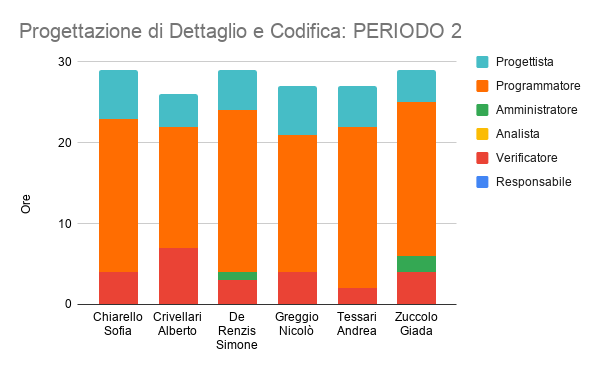
\includegraphics[scale=0.6]{res/images/charts/consuntivo/prog_dett_2.png}
	\caption{Distribuzione oraria per componente: consuntivo - Progettazione di Dettaglio e Codifica - Periodo 2}
\end{figure}


Il periodo\textsubscript{G} chiude in \textbf{positivo}, con un risparmio di \textbf{13 \euro} rispetto a quando preventivato all'inizio del periodo\textsubscript{G}. Le attività di codifica si sono svolte con efficienza e hanno permesso il risparmio di diverse ore pro-capite.


\paragraph{Preventivo a finire}
\subparagraph*{}

\pafTable{
	Avvio & 1 & Consuntivo & 1060
\tabularnewline
Analisi dei Requisiti & 1 & Consuntivo & 3380
\tabularnewline
Analisi dei Requisiti & 2 & Consuntivo & 255
\tabularnewline
Progettazione Architetturale & 1 & Consuntivo & 2220
\tabularnewline
Progettazione Architetturale & 2 & Consuntivo & 2000
\tabularnewline
Progettazione Architetturale & 3 & Consuntivo & 150
\tabularnewline
Progettazione di Dettaglio e Codifica & 1 & Consuntivo & 909
\tabularnewline
Progettazione di Dettaglio e Codifica & 2 & Consuntivo & 2760
\tabularnewline
Progettazione di Dettaglio e Codifica & 3 & Preventivo di periodo & 280
\tabularnewline
Validazione e Collaudo & 1 & Preventivo & 220
\tabularnewline
Validazione e Collaudo & 2 & Preventivo & 2145
\tabularnewline
Validazione e Collaudo & 3 & Preventivo & 60
\tabularnewline
\textbf{Totale} & \textbf{} & \textbf{} & \textbf{15439}
\tabularnewline
\textbf{Totale rendicontato} & \textbf{} & \textbf{} & \textbf{10744}
\tabularnewline
\caption{Preventivo a finire - Progettazione di Dettaglio e Codifica - Periodo 2}
}

Grazie all'efficientamento delle spese operato negli ultimi periodi, è stato possibile rientrare nel preventivo iniziale.


\pagebreak
\subsection{Periodo 3}

\subsubsection{Pianificazione preventiva}

\paragraph{Attività}
\subparagraph*{}

\planningTable{
	Preparazione alla presentazione & Viene preparato il materiale necessario alla presentazione. & 7 & Amministratore
\tabularnewline 
Verifica dei macro periodi precedenti & Il gruppo si vede coinvolto in un confronto dal quale vorranno emergere le criticità riscontrate nel macro periodo\textsubscript{G} trascorso, al fine di migliorare lo svolgimento dei periodi successivi. & 1 & Responsabile
\tabularnewline 
Approfondimento personale & Ogni membro del gruppo spende alcune ore per formare e consolidare una conoscenza di base degli strumenti e tecniche da impiegare nel periodo\textsubscript{G} successivo. & 4 & Progettista
\tabularnewline 
\caption{Pianificazione preventiva - Progettazione di Dettaglio e Codifica - Periodo 3}
}

\paragraph{Preventivo}
\subparagraph*{}

\hspace{-1cm}
\begin{minipage}{.50\textwidth}
\smallPreventivoTable{
	Responsabile & 1 & 30\\ 
Verificatore & 0 & 0\\ 
Analista & 0 & 0\\ 
Amministratore & 7 & 140\\ 
Programmatore & 0 & 0\\ 
Progettista & 4 & 88\\ 
\hlinetable 
\textbf{Totale} & \textbf{12} & \textbf{258}\\ 
\end{tabular} 
\caption{Preventivo - Progettazione di Dettaglio e Codifica - Periodo 3}
}
\end{minipage}
\hspace{1cm}
\begin{minipage}{.40\textwidth}
\begin{figure}[H]
	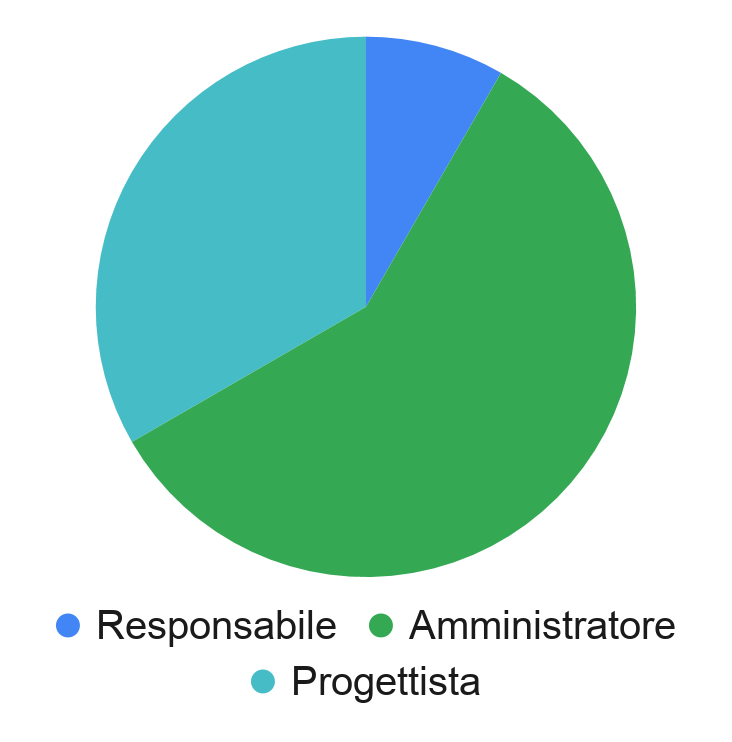
\includegraphics[scale=0.21]{res/images/charts/preventivo_priori/Grafico4-8.png}
	\caption{Distribuzione dei costi: preventivo - Progettazione di Dettaglio e Codifica - Periodo 3}
\end{figure}
\end{minipage} 



\subsubsection{Pianificazione di periodo}

%TODO: NICOLO'
%\begin{figure}[H]
%	\centering
%	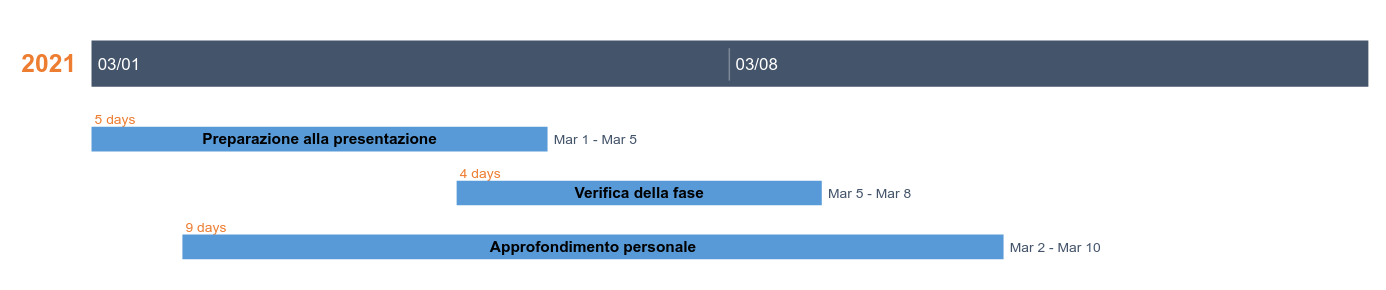
\includegraphics[scale=0.30]{res/images/gantt_periodo/progarch_3_gantt.png}
%	\caption{Gantt di periodo\textsubscript{G} - Progettazione di Dettaglio e Codifica - Periodo 2}
%\end{figure}

\paragraph{Attività}
\subparagraph*{}

\planningTable{
	Preparazione alla presentazione & Viene preparato il materiale necessario alla presentazione. & 7 & Amministratore
\tabularnewline 
Verifica dei macro periodi precedenti & Il gruppo si vede coinvolto in un confronto dal quale vorranno emergere le criticità riscontrate nel macro periodo trascorso, al fine di migliorare lo svolgimento dei periodi successivi. & 1 & Responsabile
\tabularnewline 
Approfondimento personale & Ogni membro del gruppo spende alcune ore per formare e consolidare una conoscenza di base degli strumenti e tecniche da impiegare nei periodi successivi. & 5 & Progettista
\tabularnewline 
\caption{Pianificazione di periodo - Progettazione di Dettaglio e Codifica - Periodo 3}
}



\paragraph{Preventivo orario ed economico}
\subparagraph*{}

\contabilitaTable{
	Chiarello Sofia & 1 & 0 & 0 & 1 & 0 & 0 & \textbf{2}\\ 
Crivellari Alberto & 0 & 0 & 0 & 1 & 0 & 1 & \textbf{2}\\ 
De Renzis Simone & 0 & 0 & 0 & 1 & 0 & 1 & \textbf{2}\\ 
Greggio Nicolò & 0 & 0 & 0 & 1 & 0 & 1 & \textbf{2}\\ 
Tessari Andrea & 0 & 0 & 0 & 2 & 0 & 1 & \textbf{3}\\ 
Zuccolo Giada & 0 & 0 & 0 & 1 & 0 & 1 & \textbf{2}\\ 
\hlinetable 
\textbf{Totale orario} & \textbf{1} & \textbf{0} & \textbf{0} & \textbf{7} & \textbf{0} & \textbf{5} & \textbf{13}\\ 
\textbf{Totale costo} & \textbf{30} & \textbf{0} & \textbf{0} & \textbf{140} & \textbf{0} & \textbf{110} & \textbf{280}\\ 
\end{tabular} 
\caption{Preventivo di periodo\textsubscript{G} - Progettazione di Dettagli e Codifica - Periodo 3}
}

\begin{figure}[H]
	\centering
	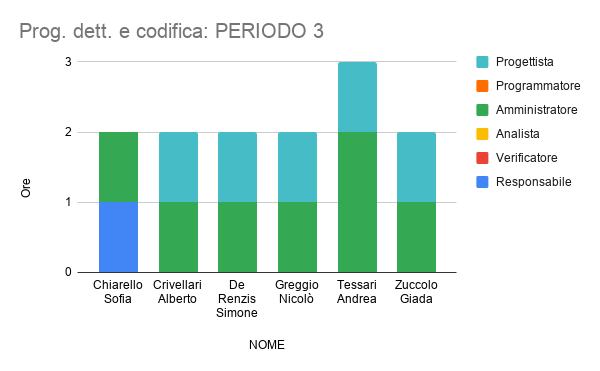
\includegraphics[scale=0.6]{res/images/charts/preventivo/prog_dett_3.png}
	\caption{Distribuzione oraria per componente: preventivo di periodo\textsubscript{G} - Progettazione di Dettaglio e Codifica - Periodo 3}
\end{figure}



\subsubsection{Riscontro di fine periodo}


L'avanzamento del progetto\textsubscript{G} non prevede ancora la valorizzazione di questa sezione.
